\documentclass{article}
\usepackage[spanish]{babel}
\usepackage[utf8]{inputenc}
\usepackage[T1]{fontenc}
\usepackage{graphicx}
\usepackage{listings}
\usepackage[numbers,sort&compress]{natbib}

\title{\bf Práctica 3: teoría de colas}
\date{\today}
\author{C. A. Estrada}

\begin{document}

\maketitle

\section{Objetivo}
Examinar las diferencias en los tiempos de ejecución en distintos ordenamientos de números primos y no primos de un vector de entrada \cite{dra}, que contene números primos descargados de https://primes.utm.edu/lists/small/millions/ y no primos de al menos ocho dígitos, así como investigar el efecto de la proporción de éstos.

\section{Metodología}
Se utiliza el paquete estadístico R versión 4.0.2 \cite{R} para generar el código. Primero, se determina el número de núcleos disponibles en el sistema para que se realice la paralelización; en el presente caso, el sistema utilizado solamente posee dos núcleos, por lo que la variación de núcleos asignados al cluster no es posible.
\begin{lstlisting}[language=R]
> library(parallel)
> detectCores()
[1] 2
\end{lstlisting}
Posteriormente, se genera el código que examina el tiempo de ejecución \cite{dra}\cite{clara}, bajo distintos órdenes de números primos y no primos. Para ello se crea un vector que contenga a los números primos descargados, de los cuales se seleccionaron los últimos 2400 números primos (desde 15446071 hasta 15485863) y posteriormente se crea un segundo vector a partir de éste, sumándole 1 para volver a dichos números pares, de manera que dejen de ser primos y que sean de ocho dígitos, y con ello se genera un tercer vector de trabajo de 4800 números primos y no primos, compuesto por los dos vectores anteriores.
\begin{lstlisting}[language=R]
numprimos=read.csv("primes1-fragm.txt",header=FALSE)
noprimos=numprimos+1 
trabajo=c(numprimos,noprimos)
\end{lstlisting}
A partir de la rutina que examina si un número es primo o no \cite{dra}, se calcula el tiempo de ejecución de dicho algoritmo para el vector de trabajo, realizando diez réplicas y generando tres ordenamientos distintos: el orden original (primero los primos y luego los no primos), el invertido (primero los no primos y luego los primos) y el aleatorio.  Finalmente, se realiza un gráfico de los tiempos de ejecución obtenidos y además se obtienen los datos de estadística descriptiva.

\section{Resultados y discusión}
Los tiempos de ejecución promedio están registrados en el cuadro \ref{tabla}, en donde se observa que el orden original tuvo el menor tiempo de ejecición promedio, seguido por el orden aleatorio, mientras que el orden invertido obtuvo el mayor promedio. 
\begin{table}[h]
\begin{center}
\caption{Resumen estadística descriptiva}
\label{tabla}
\begin{tabular}{c c c c c c c}
\hline
\textbf{Ordenamiento}&\textbf{Mín.}&\textbf{1er. Qu.}&\textbf{Mediana}&\textbf{Media}&\textbf{3er. Qu.}&\textbf{Máx.}\\
\hline
Original (ot)&14.34&20.08&20.25&19.76&20.41&21.22\\
Invertido (it)&19.98&20.09&20.27&20.43&20.45&21.58\\
Aleatorio (at)&19.97&20.04&20.11&20.21&20.41&20.58\\
\hline
\end{tabular}
\end{center}
\end{table}

Tomando en cuenta que el porcentaje de números primos y no primos es el mismo (50/50), además que el ordenamiento no es una distribución uniforme en los órdenes original e invertido y que el promedio se ve afectado por valores excepcionales obtenidos en alguna repetición (como las anomalías que se observan en la figura \ref{figura1}, las cuales representan los valores mínimos y máximos obtenidos en los experimentos), se considera a la mediana como el valor que refleja mejor el comportamiento de los datos, en este caso el tiempo de ejecución. Entonces, el orden aleatorio es aquel que tarda menos en ser ejecutado, seguido por el orden original, y finalmente, el orden invertido.
\begin{figure}[ptb]
\begin{center}
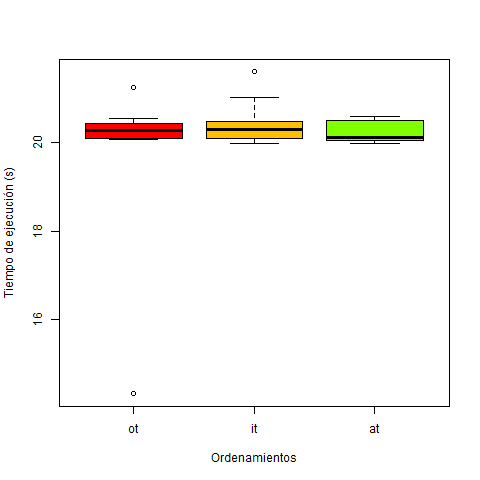
\includegraphics[width=\linewidth]{p3.png}
\end{center}
\caption{Tiempos de ejecución según el ordenamiento. Original (ot), invertido (it) y aleatorio (at).\label{figura1}}
\end{figure}

\section{Conclusión}
Con base en los datos de estadística descriptiva obtenidos a partir de los tiempos de ejecución, el orden invertido de números no primos y primos es el que obttuvo un mayor tiempo de ejecución. 

\bibliography{P3}
\bibliographystyle{unsrtnat}

\end{document}





